% file: 3-9-connectivity/menger-theorem-case-III.tex
% Based on the proof of the book ``A First Course in Graph Theory'' by Gary Chartrand and Ping Zhang

\documentclass[tikz]{standalone}
\usetikzlibrary{positioning, shapes, fit, decorations.pathmorphing}

\begin{document}
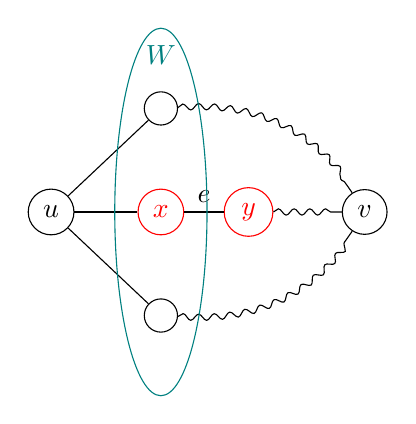
\begin{tikzpicture}[v/.style = {draw, circle, minimum size = 12pt},
  every edge/.style = {draw},
  path/.style = {-, decorate, decoration = {snake, amplitude = .4mm, segment length = 2mm, post length = 1mm}},
  vc/.style = {draw, teal, ellipse}]
  \node (u) [v] {$u$};

  \node (x) [v, right = 0.80cm of u, red] {$x$};
  \node (y) [v, right = 0.50cm of x, red] {$y$};
  \node (w1) [v, above = 0.80cm of x] {};
  \node (w3) [v, below = 0.80cm of x] {};

  \node (v) [v, right = 2.00cm of x] {$v$};

  \path (u) edge (w1)
  	    edge (x)
  	    edge (w3)
	(w1) edge[path, bend left] (v)
	(x) edge node [above] {$e$} (y)
	(y) edge[path] (v)
	(w3) edge[path, bend right] (v);

  \node (w) [vc, fit = (w1) (x) (w3), label = {[below = 3pt, teal] $W$}] {};
\end{tikzpicture}
\end{document}
